\chapter{Einleitung}
\label{cha:Einleitung}

\section{Motivation}


Die vorliegende Arbeit wurde im Rahmen einer Kooperation zwischen der Klinik für Hämatologie des Universitätsklinikums Gießen und Marburg (Molekularbiologisches Spezialroutine Labor, Leitung PD Dr. C. Brendel)\footnote{\url{https://www.uni-marburg.de/fb20/haematoonkol/forschung/brendel}} und dem Institut für Bioinformatik und Systembiologie der Justus-Liebig-Universität Gießen (Prof. Dr. A. Goesmann)\footnote{\url{https://www.uni-giessen.de/fbz/fb08/Inst/bioinformatik}} durchgeführt. 

%Die vorliegende Masterarbeit ist Teil des Forschungsfeldes der Arbeitsgruppe Brendel\footnote{\url{https://www.uni-marburg.de/fb20/haematoonkol/forschung/brendel}}, des \emph{Universitätsklinikums Gießen und Marburg}, welche sich mit \ac{AML} befasst, in Kooperation mit der \emph{Bioinformatics and Systems Biology Group} der Justus-Liebig-Universität Gießen\footnote{\url{https://www.uni-giessen.de/fbz/fb08/Inst/bioinformatik}}. 

Ziel dieser Arbeit ist es zu testen, ob die Theorie der \ac{APs} zur Annotation von \ac{SNP}s, in spezifischen Regionen, im Genom von \ac{AML} Patienten, angewendet werden kann.

Bei den \ac{APs} handelt es sich um eine Methode der Transformation, der physikochemischen und wechselwirkenden Eigenschaften, der Lage von Aminosäureseitenketten im Raum und ihrer relative Positionen zueinander, in ein Energiemaß. 
%Proteinstruktur
So können 3D-Strukturinformationen in eindimensionale Energiewerte überführt werden, mit denen leichter gerechnet werden kann. Diese jeweiligen Energiewerte der Proteine liegen in sogenannten \ac{EP}s vor und können als Grundlage für proteomische Untersuchungen dienen. Die Theorie hinter den Aminosäurerest-Pseudopotentialen existiert schon länger \cite{Heinke.2011}, jedoch wurde sie bisher nicht zur Annotation von potentiell pathogenen \ac{SNP}s eingesetzt. Die Theorie ermöglicht es uns, mehr Informationen aus der Proteinstruktur verwenden zu können, da im biologischen Kontext die korrekte Faltung der Proteine eine sehr wichtige Rolle spielt. Ein Austausch einer Aminosäure könnte somit die Faltung verändern und das Protein beschädigen. 

Bisher ist die Abfolge der Aminosäuresequenz die größte Informationsquelle etablierter proteomischer Analyseverfahren \cite{Landels.2015}. Diese jedoch spiegelt nur einen Teil der gesamten biologischen Information der Polypeptidkette wieder. Um ein tiefer gehendes Verständnis für das biologische System zu entwickeln ist es notwendig, alle möglichen Informationen einfließen zu lassen, auch die 3D-Struktur. Die Verwendung der 3D-Struktur führt jedoch zu einem drastisch erhöhten Aufwand, weswegen es bisher in den meisten Fällen nicht praktikabel war. Durch die \ac{APs} lässt sich dieser Mehraufwand erheblich verringern, indem die bisherige Aminosäuresequenz durch \ac{EP}s erweitert wird. Diese Energieprofile stellen ein eindimensionales Maß dar, welches den Rechenaufwand reduziert. Zudem sind sie leichter zu lesen und zu interpretieren, sodass die 3D-Strukturinformationen für die Analysen nutzbar sind.

In einer vorherigen Arbeit mit dem Titel \emph{Entwicklung mole\-kular-phylo\-genetisch\-er Methoden auf Grundlage von Aminosäurerest- Pseudopotentialen}, wurde gezeigt, dass es möglich ist, die Information der 3D-Strukturen, aus der \ac{PDB} und \ac{Pfam} zu nutzen \cite{Mathias.2014}. Um aus der Proteinstruktur, mit den Informationen aus den EPs eine Substitutionsmatrix zu kalkulieren, welche die zusätzlichen Informationen der \ac{APs} nutzbar macht. Es wurde durch den Vergleich mit anderen Substitutionsmatritzen gezeigt, dass \ac{EP}s mindestens äquivalent zu den etablierten Ansätzen, wenn nicht sogar besser sind. Als Fazit dieser Arbeit wurde festgehalten, dass sich \ac{EP}s als Datengrundlage eignen, um den Informationsgehalt von einfachen Sequenzen zu erweitern.

\begin{figure}
\centering
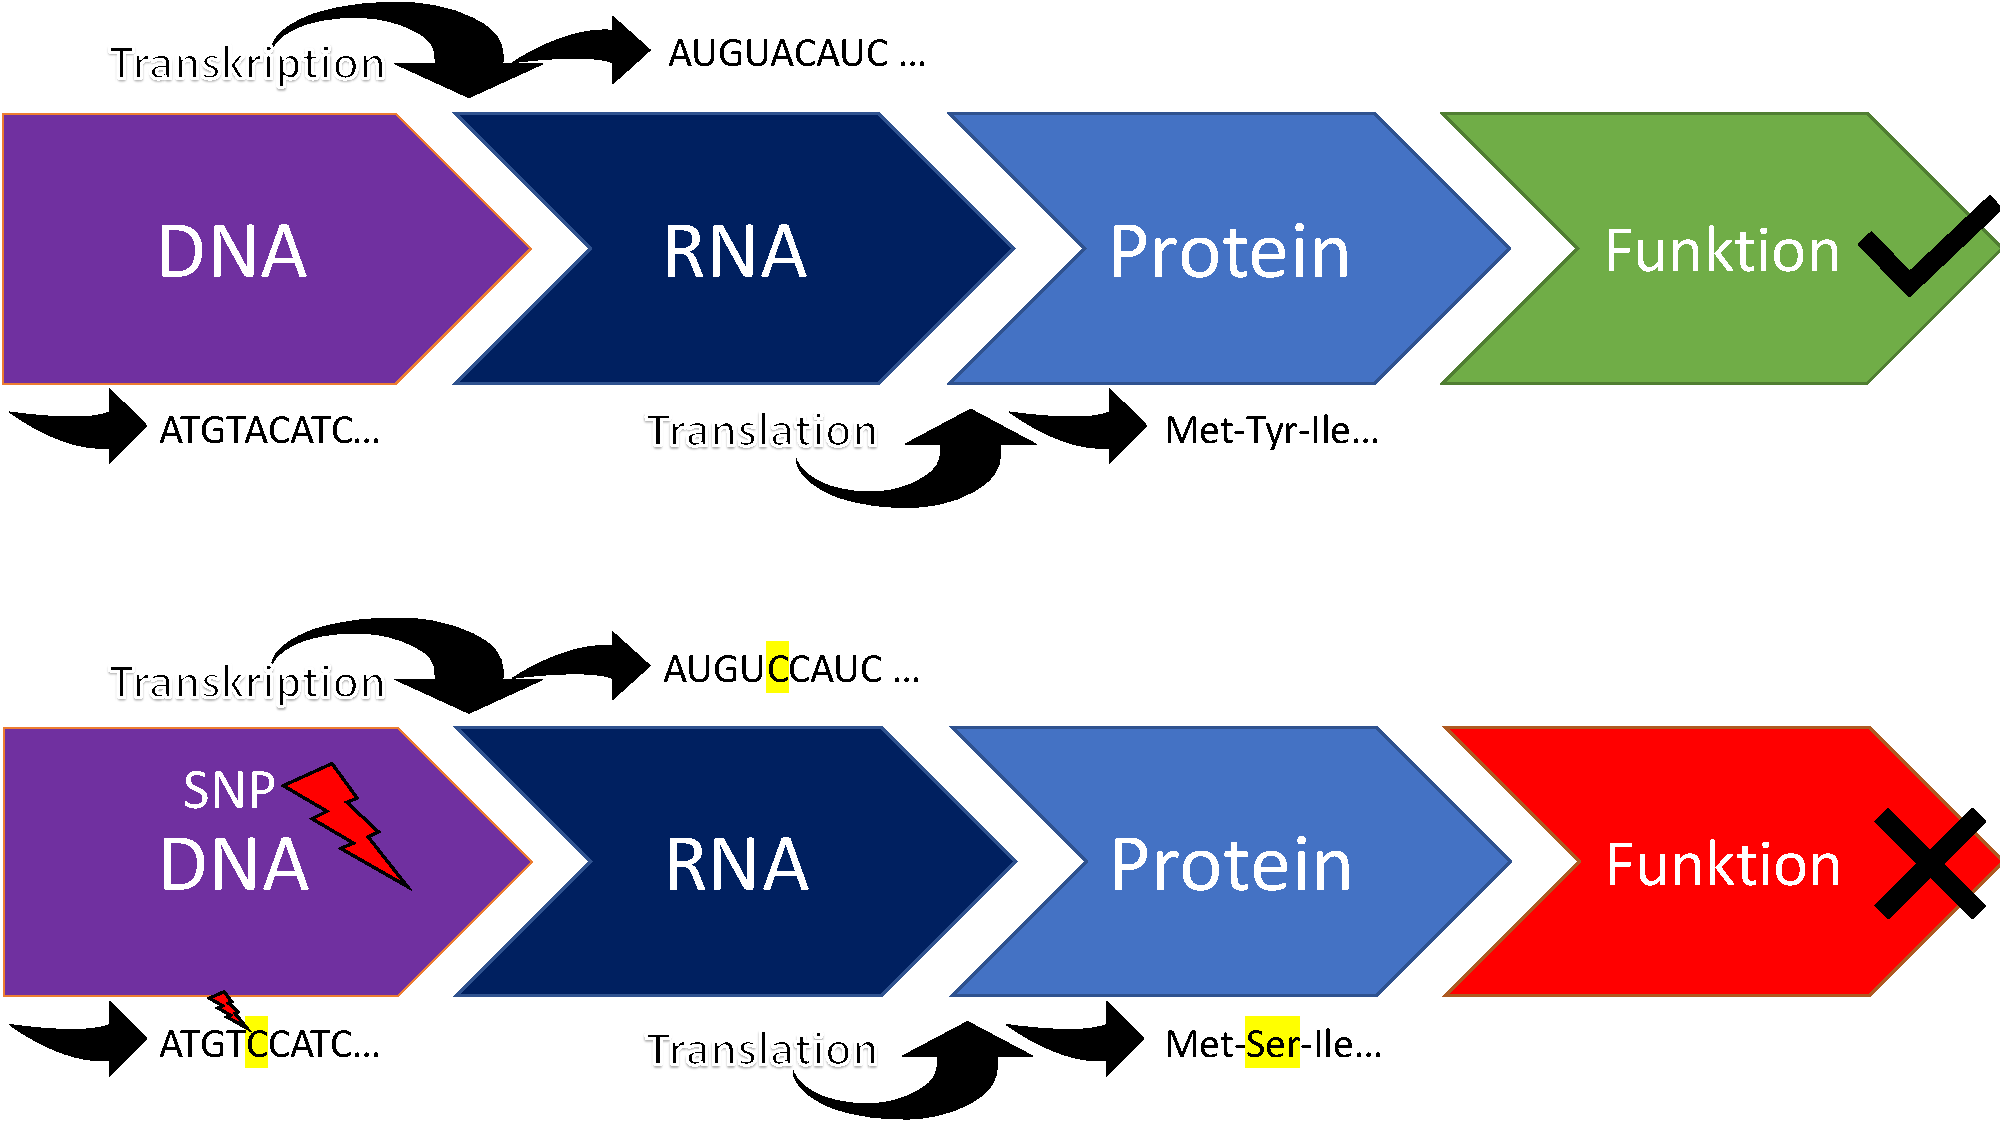
\includegraphics[width=.95\textwidth]{images/Biologie_dogma.pdf}
\caption{Das Zentrale Dogma der Biologie, aus DNA wird, mittels Transkription, RNA erzeugt. Protein wird aus RNA mittels Translation erzeugt. Jedes Protein hat eine Funktion. Wird jetzt die DNA durch einen \ac{SNP} verändert, so verändert sich die RNA, welche wiederum das Protein verändert, sodass die Funktion des Proteins gestört wird.}
\label{fig:dogma}
\end{figure}



\section{Leukämie}
\label{sec:leuk}
Leukämie ist entweder eine maligne Erkrankung des Knochenmarks bzw. des blutbildenden Systems oder des lymphatischen Systems. Es wird aktuell in vier Unterarten der Leukämie unterschieden, der Plasmazellenleukämie, der lymphatischen Leukämie, der Monozytenleukämie und der myeloischen Leukämie. Zudem gibt es eine Unterteilung in eine \emph{chronische}, meist mehrere Jahre andauernde Erkrankung und eine \emph{akute} Erkrankung, welche eine schnelle und aggressive Form darstellt.

Die Leukämie wird nach der Art der beteiligten Zellen klassifiziert. Patienten mit \ac{AML} haben eine Störung der Myelopoese, welche für die Bildung von Granulozyten, Monozyten, Erythrozyten und Megakaryozyten zuständig ist. Eine \ac{ALL} betrifft hingegen die Lymphozyten und deren Vorläuferzellen. Die Blutstammzellen verlieren bei \ac{AML} die Fähigkeit sich in Blutzellen auszudifferenzieren, zudem proliferieren sie unkontrolliert im Knochenmark \cite{Papaemmanuil.2016}. Schließlich treten undifferenzierte \emph{Blasten} (auch Leukämiezellen genannt) aus dem Knochenmark ins periphere Blut über und verdrängen dort die gesunden Zellen. Durch diese Verdrängung der normalen Blutbestandsteile entsteht ein Mangel an Sauerstoff, eine sogenannte Anämie. Weitere Symptome können ein Gefühl der Erschöpfung, Blutarmut, Hämatome und eine Schwächung des Immunsystems sein. Die \ac{AML} ist eine lebensbedrohliche Krankheit und ist unbehandelt innerhalb weniger Wochen letal. Zusätzlich können Blasten noch andere Organe, wie Leber, Milz und Lymphknoten befallen und so deren Funktionen stören.

\begin{figure}
\centering
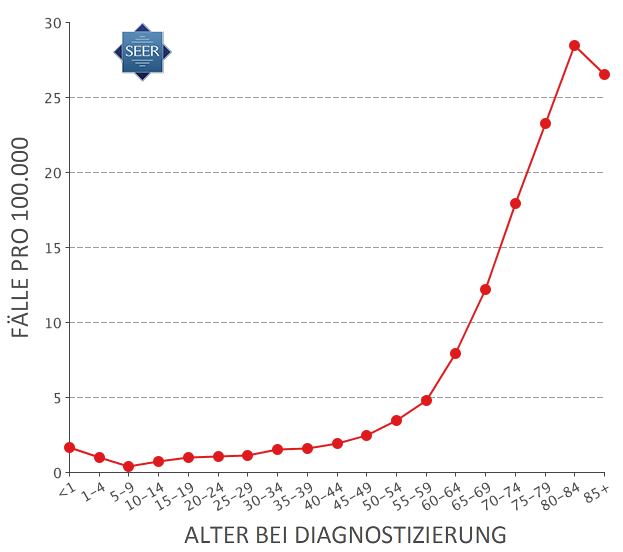
\includegraphics[width=.90\textwidth]{images/Alter_AML_2014.png}
\caption{Zu sehen ist das Auftretens einer \ac{AML} pro 100.000 Menschen, in Abhängigkeit vom Alter (in Jahren), übergreifend über alle Abstammungen und Geschlechter. \ac{Abb} geändert nach SEER \cite{Howlader.2014} Explorer\protect\footnotemark{} von 2010 bis 2014.}
\label{fig:Alter_AML}
\end{figure}
\footnotetext{\url{https://seer.cancer.gov/explorer/}}
Eine Leukämie kann in jeder Altersstufe auftreten. Doch es gibt spezifische Altersgruppen, in denen spezielle Arten der Leukämie wahrscheinlicher sind, siehe \ac{Abb} \ref{fig:Age_AML_ALL}. So tritt im Kindesalter hauptsächlich \ac{ALL} auf \cite{Rubnitz.2012}, im Erwachsenenalter ist eine \ac{AML} die wahrscheinlichste Erkrankung und im Alter (ab 50 Jahre) hat die \ac{CLL} die höchste Prävalenz, siehe \ac{Abb} \ref{fig:Alter_AML}. Generell lässt sich sagen, dass die Wahrscheinlichkeit an einer Leukämie zu erkranken, sich mit dem Alter erhöht, geschuldet durch Mutationen, die sich im Laufe des Lebens in den Zellen akkumulieren.

Die Diagnostik einer Leukämie wird durch die Klassifikation der Blasten ermöglicht, indem die morphologischen Eigenschaften der Blasten untersucht werden. Dafür wird dem Patienten eine Blutprobe entnommen und unter dem Mikroskop analysiert. Ausschlaggebend für eine Diagnostik ist unter anderem der Grad der Differenzierung, denn bei chronischen Leukämien lassen sich vermehrt Blutzellen beobachten, welche fast komplett ausdifferenziert sind, wohingegen bei einer akuten Leukämie vor allem undifferenzierte Blutzellen zu beobachten sind\footnote{\url{https://www.cancer.org/cancer/acute-lymphocytic-leukemia/about/what-is-all.html}}. Um eine endgültige Diagnose zu stellen, ist aber immer eine Knochenmarkspunktion nötig. Neben den morphologischen Eigenschaften werden die Zellen zusätzlich molekularbiologisch untersucht, indem zur Risikoeinstufung der Karyotyp bestimmt wird. Zusätzlich in den meisten Krankenhäusern eine Mutationsanalyse von ausgewählten Genen wie z.B. \texttt{FLT3, IDH1, KRAS} \& \texttt{NRAS} des Illumina TruSight Myeloid Sequencing Panel vollzogen.

\begin{figure}
\centering
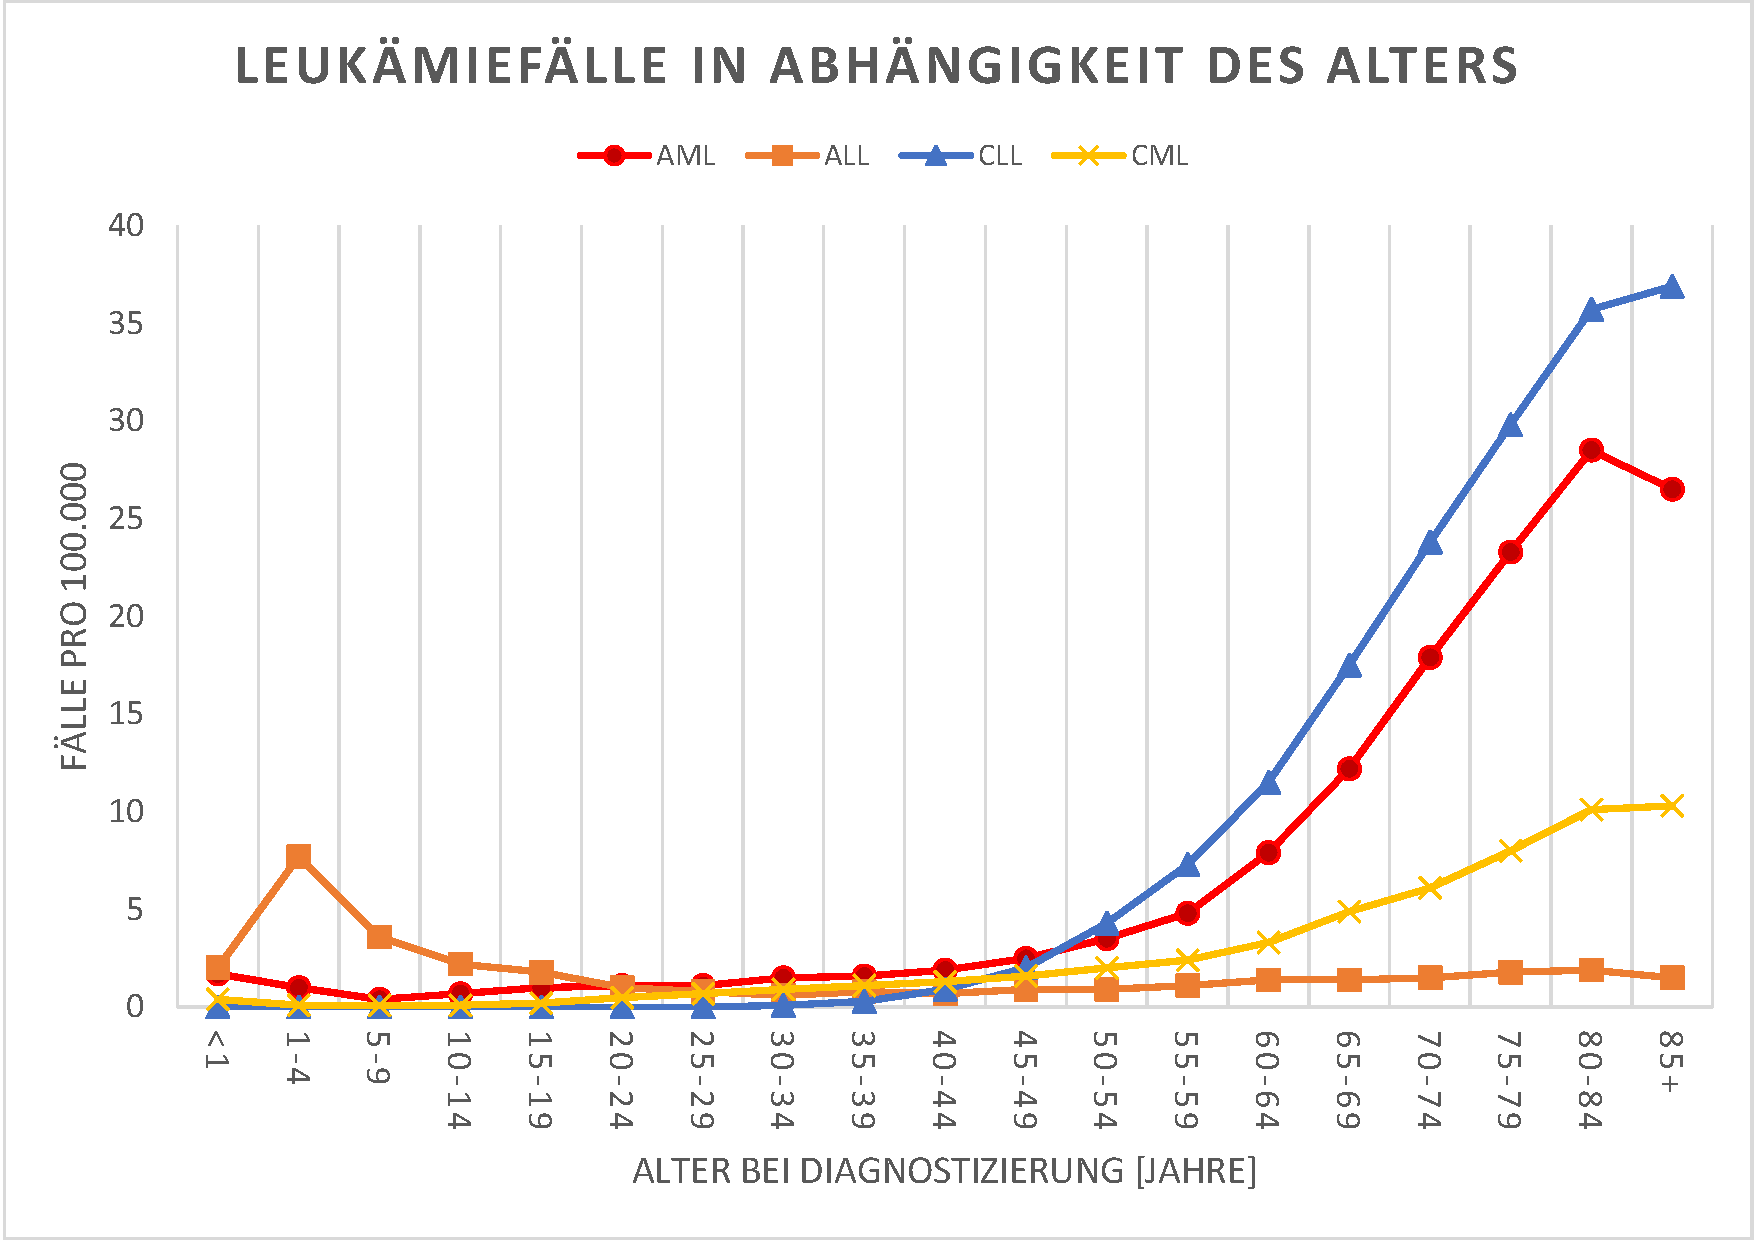
\includegraphics[width=.99\textwidth]{images/Age_AML_ALL.pdf}
\caption{Dargestellt ist das Auftretens einer speziellen Leukämie pro 100.000 Menschen in Abhängigkeit zum Alter unabhängig vom Geschlecht oder der Abstammung. Daten aus dem SEER 2010-2014.}
\label{fig:Age_AML_ALL}
\end{figure}

Leukämie entsteht durch genetische Veränderungen in undifferenzierten Blutstammzellen. Wenn die Mutationen in speziellen Regionen liegen \cite{Wakita.2016}, so teilen sich die Zellen unkontrolliert und sind in ihrer Funktion stark eingeschränkt. Es genügt bereits eine kleine Veränderung in einer der Stammzellen, damit deren Tochterzellen die gesunden Zellen verdrängen. Die Ursachen für diese genetische Modifikation sind im Großen noch unbekannt, im Allgemeinen wird jedoch vermutet, dass die spezifischen Risikofaktoren, welche Krebs begünstigen, auch eine Leukämie verursachen können \cite{Petit.2014}. Durch die technische Weiterentwicklung der Länder und der damit verbundenen erhöhten Population und Lebensspanne der Menschen, steigt die Anzahl der Krebserkrankungen. Hierbei spielen Alter, Rauchen, Übergewicht, sportliche Aktivität und Reproduktionsverhalten, geprägt durch die Urbanisierung, eine zentrale Rolle \cite{Torre.2015}. Des Weiteren steht die Aussetzung spezieller Strahlung, z.B. ionisierende Strahlung oder passive Radon Strahlung, sowie mutagene Chemikalien, diverse Viren und genetische Vorbelastung, im Verdacht krebserregend zu sein.

Therapiert wird \ac{AML} mit Zytostatika und einer allogenen Knochenmark- bzw. Stammzelltransplantation \cite{Cheson.2003}. Bei der Stamm\-zell\-trans\-plan\-tat\-ion wird das erkrankte Knochenmark durch gesunde Zellen von einem passenden Spender ersetzt. Die Stammzellen werden dem Spender, nach einer Medikation, aus dem Blut extrahiert und dem Empfänger, nach einer Chemotherapie oder Bestrahlung, mittels Transfusion, übertragen. 

Nach Therapiebeginn sind die Leukämiezellen nicht mehr unter dem Mikroskop nachweisbar. Die Molekulargenetik bietet daher die Möglichkeit, den Erkrankungsverlauf durch die Bestimmung der so genannten minimalen Resterkrankung \ac{MRD} zu verfolgen. Durch die \ac{MRD} lassen sich Leukämiezellen schon ab 0,01\% im Blut nachweisen, zum Vergleich bei morphologischen Untersuchungen liegt die Grenze bei 5\% \cite{Ossenkoppele.2016}.

Nach einer Therapie gehen die meisten Patienten in Remission, dies bedeutet, dass die Symptome der \ac{AML} zurückgehen und sie aus dem Krankenhaus entlassen werden können. Doch leider hat \ac{AML} eine hohe Rückfallquote, welche stark abhängig vom Alter ist. Sodass im Schnitt 5 Jahre nach der \ac{AML} Diagnose nur noch 26,9\% am Leben sind, siehe \ac{Abb} \ref{fig:seer_aml_rate}.

\begin{figure}
    \centering
    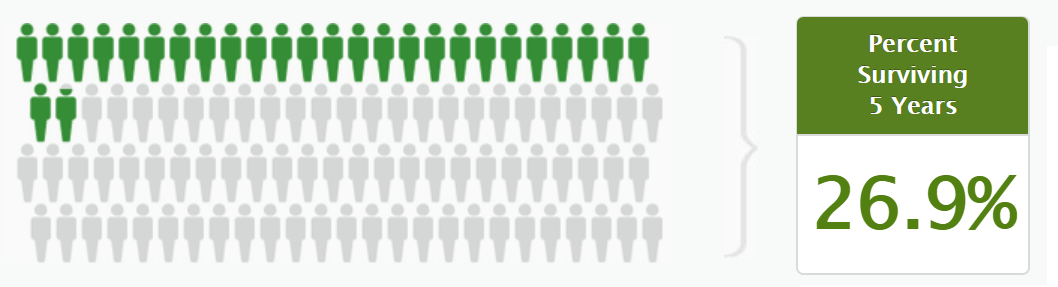
\includegraphics[width=.95\textwidth]{images/SEER_survival_rate_AML.png}
    \caption{Basierend auf Daten aus SEER 2007-2013. Graue Personen repräsentieren diejenigen, welche an \ac{AML} gestorben sind. Grüne repräsentieren diejenigen, die 5 Jahre oder mehr überlebt haben\protect\footnotemark{}.}
    \label{fig:seer_aml_rate}
\end{figure}
\footnotetext{Daten aus dem SEER \url{https://seer.cancer.gov/statfacts/html/amyl.html}}



%\section{}{Vorarbeit}
%Dieses Kapitel befasst sich mit der \ac{SNP} Annotation im allgemeinen, zusätzlich wird die Vorarbeit zu dieser Arbeit kurz vorgestellt.
\section{Einzelnukleotid-Polymorphismus}
\label{sec:snp_exp}

Bevor auf die Annotation der \ac{SNP}s eingegangen werden kann, muss erst der Begriff des Einzelnukleotid-Polymorphismus erklärt werden. Dieser kommt aus dem englischen \emph{Single Nucleotide Polymorphism} (SNP) und in wird in dieser Arbeit auch nur unter diesem Namen verwendet.

Ein \ac{SNP} ist eine genetische Variation einer Base im Genom, dies bedeutet, dass eine Base im Beispiel Abb. \ref{fig:snp} Adenin durch Thymin ausgetauscht wurde.

\begin{figure}
\centering
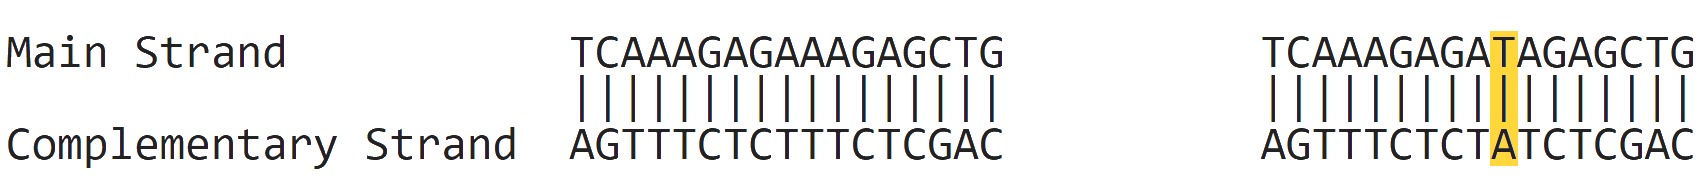
\includegraphics[width=.95\textwidth]{images/DNA_ds_strand_with_snp.png}
\caption{Doppelsträngiger DNA Ausschnitt der ABL proto-oncogene 1 tyrosine kinase mit \ac{SNP} (gelb hervorgehoben) rechts und ohne links.}
\label{fig:snp}
\end{figure}

%\begin{lstlisting}
%Leitstrang           TCAAAGAGAAAGAGCTG          TCAAAGAGATAGAGCTG
%                      |||||||||||||||||          |||||||||||||||||
%Folgestrang          AGTTTCTCTTTCTCGAC          AGTTTCTCTATCTCGAC
%\end{lstlisting}


Durch \emph{whole genome} \ac{SNP} Analysen wurde ermittelt, dass genetische Variationen zwischen menschlichen Genomen fast gänzlich durch \ac{SNP}s dargestellt werden \cite{Do.2015}. 
\ac{SNP}s können in \emph{open reading frames} (orf), aber auch in nicht codierenden Bereichen der DNA vorkommen. Einige \ac{SNP}s liegen direkt in Exons und werden in Protein translatiert. Diese Proteine können, je nach Art des \ac{SNP}s, eine veränderte Struktur und Funtktion aufweisen. Jedoch können auch nicht kodierende \ac{SNP}s das Risiko für bestimmte Erkrankungen erhöhen, z.B. beeinflussen einzelne \emph{non coding} \ac{SNP}s im Gen \emph{IKZF1} das Risiko für Kinder an ALL zu erkranken \cite{Papaemmanuil.2009}.

Es gibt verschiedene Arten von \ac{SNP}s:

\begin{description}
\item[Frameshift]
Ein \emph{Frameshift} sorgt durch eine \emph{Insertion} oder \emph{Deletion} für eine Verschiebung des Leserasters und ist fast immer pathogen.
\item[Missense]
Der häufigste Typ der \ac{SNP}s ist die sogenannte \emph{Missense variation}, hierbei wird eine Base durch eine andere ausgetauscht und ggf. auch die entstehende Aminosäure verändert, wenn sich der \ac{SNP} in einem codierenden Bereich befindet. 
\item[Nonsense]
Die \emph{Nonesense} Mutation sorgt für eine Entstehung eines termininierende Triplets, welches die Transkription vorzeitig abbricht.
\item[Splice site]
Ist ein SPN in einer \emph{splicing site}, so können einige Transkripte des Gens von dem \ac{SNP} verändert werden, während Andere nicht beeinflusst werden.
\item[ncRNA]
Wie oben erwähnt gibt es \emph{non coding} (nc) Bereiche in denen \ac{SNP}s liegen können, liegt nun ein \ac{SNP} in einem Intron, so wird es durch den Splicing Prozess herausgeschnitten und letztendlich nicht in Protein translatiert. 
\item[Near gene]
Eine weitere Besonderheit sind SNPs, welche sich in der Nähe von Genen aufhalten. Somit sollten diese nach bisherigem Wissen keinen Einfluss auf den Organismus haben, jedoch wurde gezeigt, dass es epigenetische Faktoren gibt, wie \emph{Silencer} Regionen, welche so die Expression eines Gens beeinflussen können\cite{Maston.2006}. 
\item[UTR]
UTR steht für \emph{untranslated regions} und bezeichnet den Bereich, welcher innerhalb der mRNA vor dem Start- und hinter dem Stoppcodon liegt also jenen, welcher nicht in eine Aminosäuresequenz translatiert wird.
\end{description}




\section{SNP Annotation}
\begin{sloppypar}
Um zu verstehen welche Auswirkungen ein \ac{SNP} auf den Organismus hat, ist es wichtig diesen zu annotieren. 
Für die Annotation von \ac{SNP}s existieren derzeit über 20 verschiedene verschiedene Algorithmen zur funktionellen Vorhersage: \texttt{SIFT}, \texttt{Polyphen2-HDIV}, \texttt{Polyphen2-HVAR}, \texttt{LRT}, \texttt{MutationTaster2}, \texttt{MutationAssessor}, \texttt{FATHMM}, \texttt{MetaSVM}, \texttt{MetaLR}, \texttt{CADD}, \texttt{VEST3}, \texttt{PROVEAN}, \texttt{FATHMM-MKL coding}, \texttt{fitCons}, \texttt{DANN}, \texttt{GenoCanyon}, \texttt{Eigen coding}, \texttt{Eigen-PC}, \texttt{M-CAP}, \texttt{REVEL}, \texttt{MutPred}. 
\end{sloppypar}
Außerdem gibt es noch Algorithmen, welche den Grad der Konservierung einer Position analysieren, dazu zählen: \texttt{PhyloP, phastCons, GERP++} und \texttt{SiPhy}.

Alle Algorithmen in dieser Arbeit vorzustellen wäre nicht zielführend und würde den Rahmen sprengen. Daher wird in dieser Arbeit nur auf die wichtigsten Unterschiede zwischen den Algorithmen exemplarisch eingegangen. 

\begin{figure}
\centering
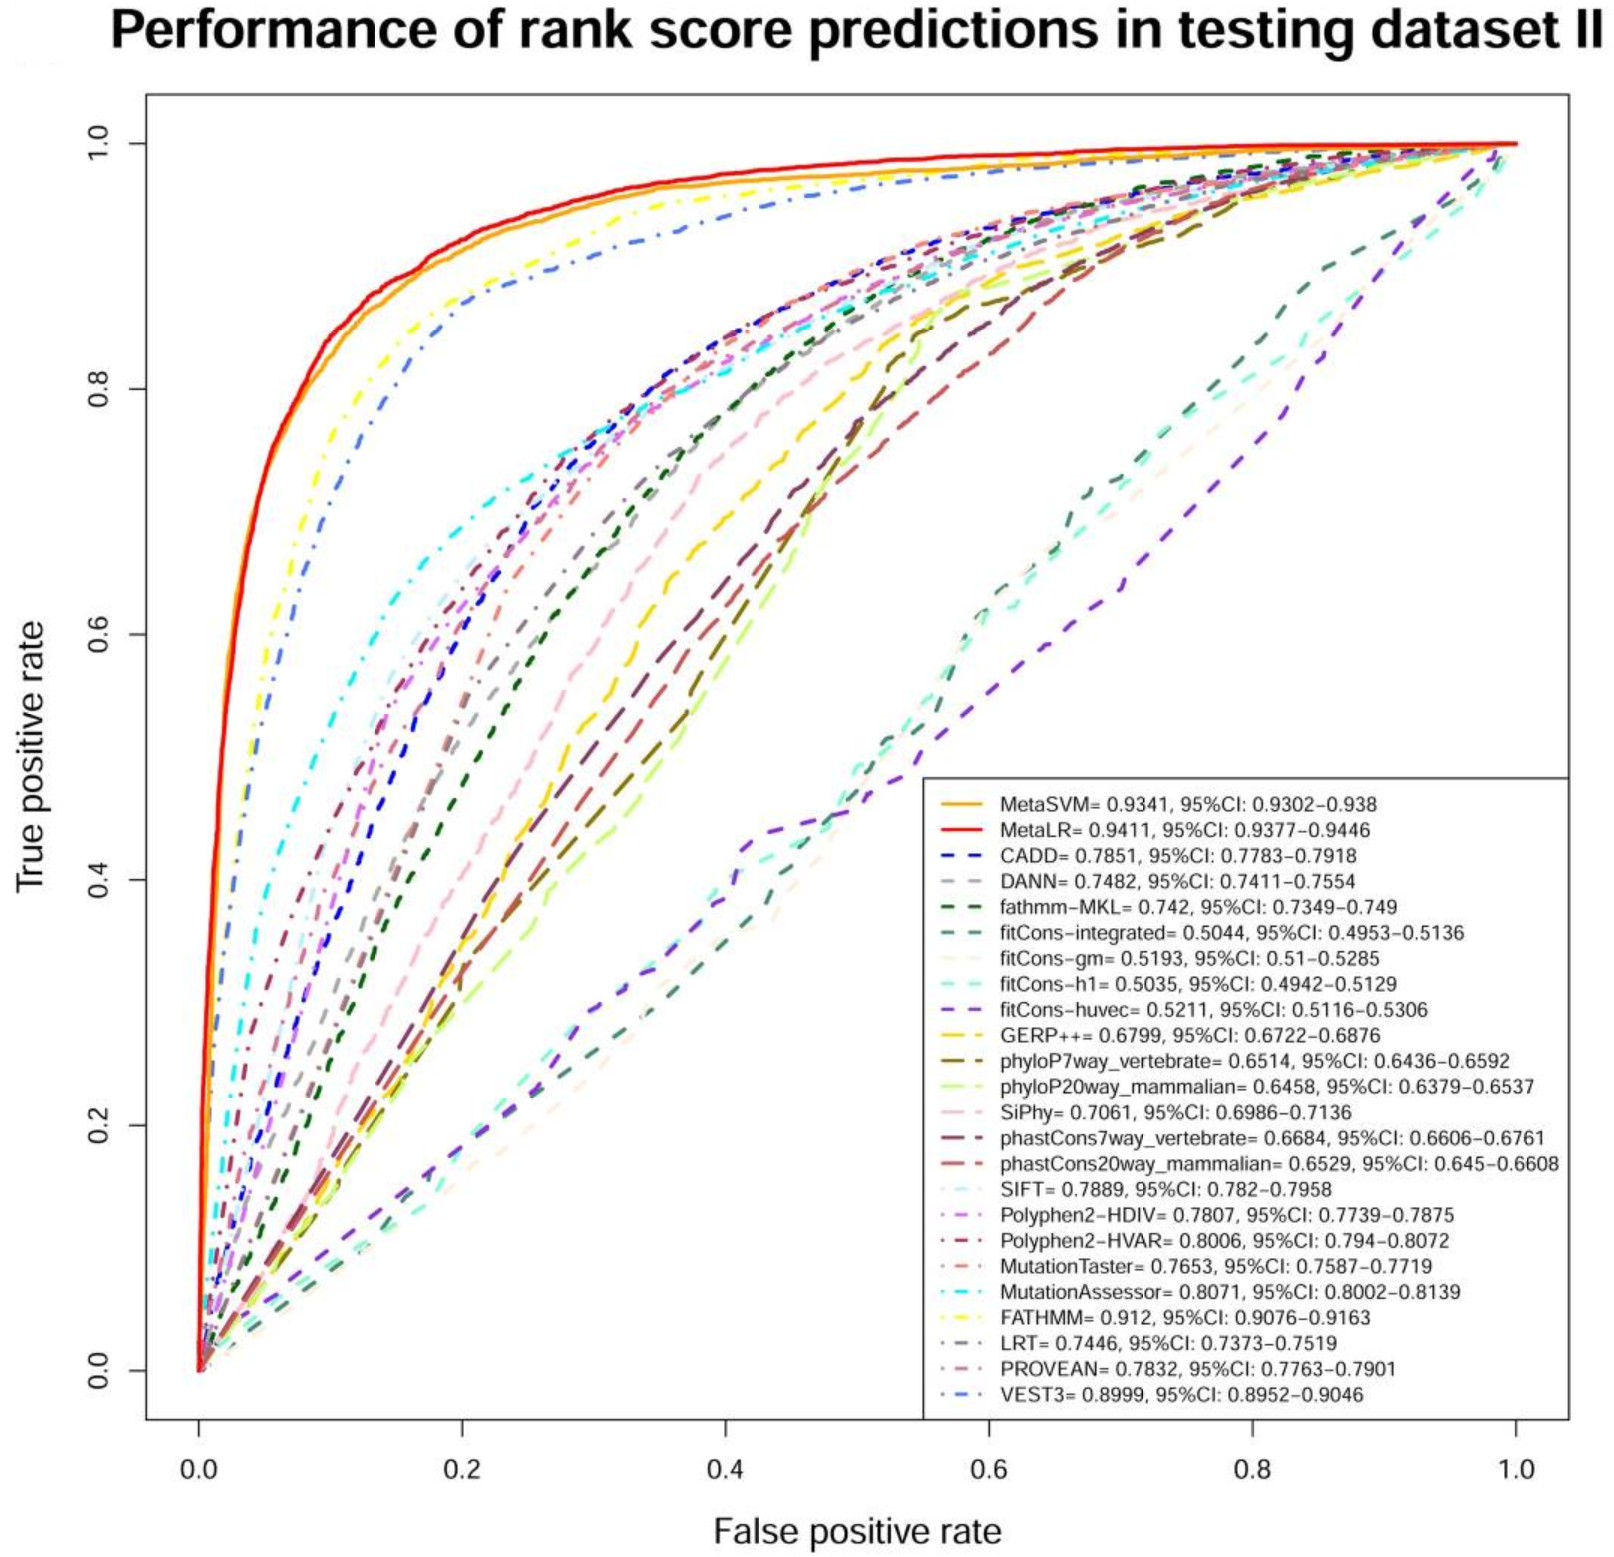
\includegraphics[width=.95\textwidth]{images/compared_prediction_scores.png}
\caption{\ac{ROC} Kurven für die funktionellen Vorhersage- und Konservierungs- Scores der dbNSFP v3.0 mit Testdatensatz II aus der Arbeit\cite{Liu.2016}. Zu sehen ist die \emph{false positive} Rate auf der Abszisse und die \emph{true positive} Rate auf der Ordinate.}
\label{fig:comp_scores}
\end{figure}

So arbeitet der \texttt{Sift}\cite{Vaser.2016} Algorithmus mit der Wahrscheinlichkeit mit der eine Aminosäure an einer Position toleriert wird, anhand von Referenz Protein Familien.
\texttt{Polyphen2}\cite{Adzhubei.2013} steht für \emph{Polymorphism phenotyping}, dieser Algorithmus arbeitet mit \emph{machine learning} und einem Trainingsdatenset \emph{HumDiv/HumVar}.
\texttt{FATHMM}\cite{Shihab.2013} steht für \emph{Functional Analysis through Hidden Markov Models} und arbeitet wie der Name schon sagt mit Hidden Markov Modellen.
Als letztes ist noch der \texttt{DANN} \cite{Quang.2015} Algorithmus erwähnenswert, dieser Arbeitet mit neuronalen Netzwerken, was sich auch in seinem Namen widerspiegelt: \emph{deleterious annotation of genetic variants using neural networks}.

Hierbei ist wichtig zu erwähnen, dass kein Algorithmus eine perfekte Vorhersage treffen kann. So wurde in der Arbeit \cite{Liu.2016} ein Trainingsdatensatz bekannter SNPs mit allen Algorithmen annotiert und das Ergebnis ausgewertet siehe \ac{Abb} \ref{fig:comp_scores}. Hierbei lieferte \texttt{MetaSVM} eine \ac{SVM} und \texttt{MetaLR} eine \ac{LR} über alle Scores, also eine Kombination aus allen Scores das beste Ergebnis.

%https://www.ncbi.nlm.nih.gov/pmc/articles/PMC4752381/ 

Zusätzlich gibt es noch eine unbestimmte Anzahl von Weiterentwicklungen und Variationen der etablierten Vorhersage Algorithmen, wie z.B. der neue \texttt{FATHMM-XF}\cite{Rogers.2017} oder \texttt{SIFT-MS}\cite{Smith.2015}.



\section{Vorarbeit}
\subsection{SNP annotation programm for AML}
\label{sec:sapa}
In einer vorherigen Arbeit wurde ein Programm namens \emph{SAPA}\footnote{\url{https://github.com/TobiasJu/SAPA}} erstellt, welches zur Annotation von \emph{Illumina truseq amplicon variants} Daten dient. Das Programm nutzt die oben erwähnten Algorithmen, allerdings aus Performancegründen nicht alle explizit, sondern nutzt die dbNSFP\cite{Liu.2016}, indem als Backend auf Annovar\cite{Wang.2010} gesetzt wird. 

Das Programm wurde am Ende mit einem ClinVar Datensatz aus 2023 pathogenen und 2000 benignen \ac{SNP}s getestet. Bei den Daten handelt es sich ausschließlich um \ac{SNP}s, welche von mehreren Autoren die gleiche Vorhersage erhalten haben. Somit sollte die bestmögliche Konsistenz gewährt sein.

Nach der Auswertung der Annotation wurde so ein \emph{MCC} von 0,64 ermittelt.


\section{Zielsetzung}

Im Universitätsklinikum Marburg, in der AG Brendel wird mit dem \emph{Illumina TruSight Myeloid Sequencing Panel}\footnote{\url{https://www.illumina.com/products/by-type/clinical-research-products/trusight-myeloid.html}} gearbeitet, um Regionen von \ac{AML} spezifischen Genen auf Mutationen zu untersuchen. Genpanelanalysen liefern eine Tabelle mit allen Mutationen des Patienten und deren Lokalisation. Dabei liegen die meisten Mutationen in Form von \ac{SNP}s vor. Viele Patienten zeigen die gleichen Symptome einer \ac{AML}, bei unterschiedlichen detektierten \ac{SNP}s, diese sind Patienten spezifisch und ihre Auswirkung noch unbekannt. Dies hat zur Folge, dass keine Aussage über eine eventuelle Pathogenität und deren Einfluss auf den Organismus getroffen werden kann.

%Ziel dieser Masterarbeit ist die Entwicklung eines Programms zur Klassifizierung von \ac{SNP}s, aus dem Illumina TruSight Myeloid Sequencing Panel mit Hilfe von \ac{APs}.
Ziel dieser Masterarbeit war die Entwicklung eines Computerprogramms zur zuverlässigen Klassifizierung der Pathogenität von SNPs, welche nicht in Datenbanken annotiert sind. Hierbei lag der Fokus auf \ac{SNP}s aus dem Illumina TruSight Myeloid Sequencing Panel.

Klassifikationen von \ac{SNP}s sind eminent wichtig, um ein Verständnis für die Ursachen von \ac{AML} zu erhalten. Jedoch liegen aktuell, in den meisten Fällen\footnote{\url{https://www.ncbi.nlm.nih.gov/clinvar/}}, keine Informationen über die Pathogenität der gefundenen \ac{SNP}s vor. In einer vorherigen Arbeit wurde ein Programm zum Annotieren von \ac{SNP}s geschrieben, jedoch liefert dieses nur einen \ac{MCC} von 0,66 und ist damit verbesserungswürdig, siehe Kapitel \ref{sec:sapa}.

Nun soll der Versuch unternommen werden, eine Annotation der \ac{SNP}s, unter Zuhilfenahme der 3D-Struktur, zu ermöglichen. Mittels des Modells der \ac{APs} soll überprüft werden, inwiefern sich \ac{EP}s als Datengrundlage für eine \ac{SNP} Annotation in diesem Forschungsbereich eignen. Zusätzlich soll mithilfe der \ac{PDB} und \ac{Pfam}, diejenigen Proteinfamilien ermittelt werden, welche eine aufgeklärte Struktur in der \ac{PDB} besitzen, um so durch \ac{SNP}s auftretende Veränderungen der PSI \& PHI Winkel, erklären zu können. 
%Letztendlich soll getestet werden in welcher Proteindomäne der \ac{SNP} liegt, z.B. in einem hoch konservierten Bereich einer Protein Familie, um auch hiermit eine Klassifikation vorzunehmen zu können.



\section{Aufbau der Arbeit}

Zu Beginn dieser Arbeit werden die Grundlagen vermittelt, welche für die Arbeit essentiell sind. Dies beinhaltet die Erläuterung der Theorie der \ac{APs} und deren mathematischer Hintergrund. Zudem beinhaltet das Kapitel die Erklärung der Datenbanken \ac{PDB} und \ac{Pfam}, welche als die Grundlage der PSI \& PHI Winkel Berechnung genutzt wurden. 
%Zusätzlich dienen die in der \ac{PDB} enthaltenen Strukturdaten als Grundlage der \ac{EP}s. 
Außerdem wird auf die Klassifizierung mittels F1 Score bzw. \ac{MCC} eingegangen, sowie der Ramachandran Plot, \emph{Homologie Moddeling} und die wichtigsten verwendeten Programmiersprachen
%und \emph{Machine Learning}
erklärt. Abschließend wird die lokale Berechnung der Energieprofile mittels Nextflow, auf dem Clusters der Bioinformatics and Systems Biology Group der Justus-Liebig-Universität Gießen, kurz vorgestellt.

Nach Vermittlung der Grundlagen, folgt ein kurzes Kapitel zu den bisherigen Erkenntnissen aus der vorangegangenen Arbeit (Kapitel \ref{sec:sapa}), als Einleitung zum Hauptteil.

Danach folgt die Konstruktion eines adäquaten Datensatzes Kapitel \ref{chap:Datenaquirierung}, anhand vorangegangener Arbeiten \cite{Mathias.2014}. Dabei wird vor allem auf die Selektion der Daten eingegangen und Schritt für Schritt erklärt wie diese erarbeitet wurden. Zusätzlich wird auf die Berechung der \ac{EP}s und der zugehörigen Kontaktmatrix eingegangen.

% Satz is zu kurz
Der Hauptteil der Arbeit beginnt mit der Analyse der Spektren der \ac{EP}s und den Berechnungen. Anschließend werden die PSI \& PHI Winkel Berechnungen vorgestellt und ausgewertet.

%%%%%%% PSI und PHI genauer %%%%%%%%%%%%%%


Abschließend werden die Ergebnisse und Erkenntnisse der Arbeit nochmals zusammengefasst, die Aussagekraft bezüglich der Anwendung von \ac{EP}s zur Annotation von \ac{SNP}s diskutiert. Und ein Ausblick gegeben was in Zukunft mit den gewonnen Erkenntnissen möglich sein könnte.


% der Klassifikation des erstellten Programms diskutiert
